\documentclass{sig-alternate}
\usepackage{multicol}
\usepackage{graphicx, epsfig}
\usepackage{graphicx}
\usepackage{url}
\begin{document}
\conferenceinfo{GECCO'15,} {July 11-15, 2015, Madrid, Spain.}
    \CopyrightYear{2015}
    \crdata{TBA}
    \clubpenalty=10000
    \widowpenalty = 10000
%
% --- Author Metadata here ---
%\conferenceinfo{WOODSTOCK}{'97 El Paso, Texas USA}
%\CopyrightYear{2007} % Allows default copyright year (20XX) to be over-ridden - IF NEED BE.
%\crdata{0-12345-67-8/90/01}  % Allows default copyright data (0-89791-88-6/97/05) to be over-ridden - IF NEED BE.
% --- End of Author Metadata ---

\title{Using evolutionary algorithms to optimize the estimation of a diffusion process}
%
% You need the command \numberofauthors to handle the 'placement
% and alignment' of the authors beneath the title.
%
% For aesthetic reasons, we recommend 'three authors at a time'
% i.e. three 'name/affiliation blocks' be placed beneath the title.
%
% NOTE: You are NOT restricted in how many 'rows' of
% "name/affiliations" may appear. We just ask that you restrict
% the number of 'columns' to three.
%
% Because of the available 'opening page real-estate'
% we ask you to refrain from putting more than six authors
% (two rows with three columns) beneath the article title.
% More than six makes the first-page appear very cluttered indeed.
%
% Use the \alignauthor commands to handle the names
% and affiliations for an 'aesthetic maximum' of six authors.
% Add names, affiliations, addresses for
% the seventh etc. author(s) as the argument for the
% \additionalauthors command.
% These 'additional authors' will be output/set for you
% without further effort on your part as the last section in
% the body of your article BEFORE References or any Appendices.

\numberofauthors{6} %  in this sample file, there are a *total*
% of EIGHT authors. SIX appear on the 'first-page' (for formatting
% reasons) and the remaining two appear in the \additionalauthors section.
%
\author{
% You can go ahead and credit any number of authors here,
% e.g. one 'row of three' or two rows (consisting of one row of three
% and a second row of one, two or three).
%
% The command \alignauthor (no curly braces needed) should
% precede each author name, affiliation/snail-mail address and
% e-mail address. Additionally, tag each line of
% affiliation/address with \affaddr, and tag the
% e-mail address with \email.
%
% 1st. author
\alignauthor
Eliminated
%Nuria Rico\titlenote{Dr.~Rico}\\
%       \affaddr{Statistics and Operational Research}\\
%       \affaddr{University of Granada}\\
%       \affaddr{Granada, Spain}\\
%       \email{nrico@ugr.es}
\alignauthor
Eliminated
%M. G. Arenas\titlenote{Dr. ~Arenas}\\
%       \affaddr{Computer Architecture}\\
%       \affaddr{University of Granada}\\
%       \affaddr{Granada, Spain}\\
%       \email{mgarenas@ugr.es}
% 3rd. author
\alignauthor
Eliminated 
%Desir\'{e}e Romero\titlenote{Dr. ~Romero}\\
%       \affaddr{Statistics and Operational Research}\\
%       \affaddr{University of Granada}\\
%       \affaddr{Granada, Spain}\\
%       \email{deromero@ugr.es}
\and  % use '\and' if you need 'another row' of author names
% 4th. author
\alignauthor
Eliminated 
%P. A. Castillo\titlenote{Dr. ~Castillo}\\
%       \affaddr{Computer Architecture}\\
%       \affaddr{University of Granada}\\
%       \affaddr{Granada, Spain}\\
%       \email{pacv@ugr.es}
% 5th. author
\alignauthor
Eliminated
%J. M. Crespo\titlenote{Dr. ~Crespo}\\
%       \affaddr{Statistics and Operational Research}\\
%       \affaddr{University of Granada}\\
%       \affaddr{Granada, Spain}\\
%       \email{crespo@ugr.es}
% 6th. author
\alignauthor
Eliminated
%J. J. Merelo\titlenote{Dr. ~Merelo}\\
%       \affaddr{Computer Architecture}\\
%       \affaddr{University of Granada}\\
%       \affaddr{Granada, Spain}\\
%       \email{jmerelo@ugr.es}
}
% There's nothing stopping you putting the seventh, eighth, etc.
% author on the opening page (as the 'third row') but we ask,
% for aesthetic reasons that you place these 'additional authors'
% in the \additional authors block, viz.
%\additionalauthors{Additional authors: John Smith (The Th{\o}rv{\"a}ld Group,
%email: {\texttt{jsmith@affiliation.org}}) and Julius P.~Kumquat
%(The Kumquat Consortium, email: {\texttt{jpkumquat@consortium.net}}).}
\date{1 Feb 2015}
% Just remember to make sure that the TOTAL number of authors
% is the number that will appear on the first page PLUS the
% number that will appear in the \additionalauthors section.

\maketitle

\begin{abstract}
Diffusion processes are stochastic models, % of what? -- JJ
 usually employed for
modeling and forecasting in observed paths that vary along time under
random environment. % Don't understand -- clarify - JJ
 Such models are useful if we are able to know the values of the
 parameters involved. The maximum likelihood estimation of the
 parameters requires a system of equations that, for some cases, has
 no explicit solution; thus, the solution needs be estimated. We will
 use optimization methods to find those solutions: an Iterative
 Method, an algorithm based on Newton-Raphson solver, a Variable
 Neighbourhood Search method, a Simulated Annealing algorithm and an
 Evolutionary Algorithm. We generate four data sets following a
 Gompertz-lognormal diffusion process using different noise
 levels. % are these data sets complete? They correspond to what? - JJ
The methods are applied to these data sets in order to
 estimate the parameters that rule the diffusion process. Results show
 that bio-inspired methods yield suitable solutions for the problem in
 all four data sets, even when the noise level increases. %noise is
                                %first mentioned here. Why is it
                                %important? - JJ
 On the other hand,
 some analytical methods as Newton-Raphson or the Iterative Method do
 not always solve the problem if their scores depend on the
 starting point for initial solution or the noise level hinders the
 resolution of the problem. In these cases, the bio-inspired
 algorithms remain  a suitable and 
reliable approach.

%\keywords{Maximum likelihood estimate, parameters estimation}
\keywords{Diffusion Process, Parameter Estimation, Optimization Methods}
\end{abstract}

\section{Introduction}

Many probabilistic models are frequently used for modelling natural
growth-patterns and making forecasts % of what? - JJ
. Although there exists a lot of
different growth-patterns, and many different ways of modeling them,
among the most widely
studied and useful models are diffusion processes. % cita - JJ
 They are frequently
employed in biological growth modelling. \cite{lognormal}. 

Diffusion process is an usual mathematical formulation of a model for population growth in a randomly
varying environment \cite{lognormal}. %again same citation?  - JJ
 These models also describe how a population adopts a new innovation, technology or behaviour \cite{Myrskyla2013}. With these kind of models, we have the transition density function (t.d.f.) which express the chance of observing
any size for the population at any time when the initial size is specified. With the t.d.f we also are able to determine the time at that population first reaches a fixed size. Moreover, we can forecast future values of the population size as well as confidence intervals for the predictions.

In this paper we focus our attention on the Gompertz-lognormal diffusion process. It can be seen as a mixture between a Gompertz-type process \cite{Gut07b} and a lognormal process \cite{GutCy}. The first one models precesses with trends showing enclosed growth patterns, as biological growth with finite space or resources. The second one is useful for modelling not bounded growth with exponential trend.

The mixture of them, the Gompertz-lognormal diffusion process, combines both trends; a first part Gompertz-like growth and a second exponential part. This process is defined through the infinitesimal moments
%{\scriptsize
\[
\begin{array}{l}
A_1(x,t)=(m e^{-\beta t}+c)x \\
A_2(x,t)=\sigma^2 x^2,
\end{array}
\]
with $m > \beta > 0$, $c\in \mathbb{R}$.
%}
%Maribel: Deber{\'\i}amos poner qu{\'e} es m, que es e, que es c y por supuesto mencionar que t es el tiempo y que x es la variable independiente no?

Taking $c=0$ the process is Gompertz-type, and for a known fixed value of $\beta$ the process is an homogeneous lognormal diffusion process. In other cases, the process has a shape with two inflection points. This makes the process useful for modeling situations with observed paths along time that turn from increasing to decreasing or from concave to convex.

To carry out the estimation, we consider the t.d.f., that depends on $m$, $\beta$, $c$ and $\sigma^2$ parameters. Estimating the set of parameters leads to the estimation of the main features of the process. The most widely used, specifically for predicting purposes, are the mean, mode and quantile functions. Their expressions depend on the set of parameters $\{m;\beta; c; \sigma^2\}$ and, in the case of a lognormal initial distribution being considered, on the $\{ \mu_1, \sigma_1^2 \}$ set too.

The problem we deal with is to find the maximum likelihood estimates
(MLE) of the parameters of the model, from which the estimation of the
parametric functions can be found. Thus, we assume $x_{ij}$,
$i=1,\cdots,d$, $j=n_1, \cdots, n_d$ a discrete sampling of $d$ paths,
observed in $n_i$ times named $t_{ij}\,(i=1,\cdots,d,j=1,\cdots,n_i
)$, not necessarily equal in each observed path, but $t_{i1}=t_{1}$,
$i=1,\cdots, d$. With the sample, we try to obtain MLE of the
parameters maximising the likelihood function, or equivalently,
maximising the log-likelihood without constants values. So the final
function we have to maximise, using $b=e^{-\beta}$, and
$k=\sum_{i=1}^d n_i$ , is equation ( \ref{funcion}). 

\begin{figure*}[htb]
\begin{equation}
\label{funcion}
L(m,b,c,\sigma^2)=\frac{d-k}{2}\ln\sigma^2
-\frac{1}{2}\sum_{i=1}^d\sum_{j=2}^{n_i}\frac{\left[\ln\frac{x_{ij}}{x_{ij-1}}-
    \frac{m}{\ln(b)} \left(b^{t_{ij}}-b^{t_{ij-1}}\right)+\left(\frac{\sigma^2}{2}-c\right)(t_{ij}-t_{ij-1})\right]^2}
    {(t_{ij}-t_{ij-1})\sigma^2}
\end{equation}
\end{figure*}

We differentiate (\ref{funcion}) with respect to all the unknown parameters, and equalize the expressions to zero to obtain the system of equations to solve. In addition, we consider the case $t_{ij}-t_{ij-1}=h$, $i=1,\ldots,d$ and rewrite the system as equation (\ref{tochoEcuacion}) obtaining, after some operations, that all the estimations depend on $b$ as equation (\ref{estima}) shows. Finally, we have the equation (\ref{ecuacion}) that has no explicit solution.



\begin{figure*}[htb]
%\begin{equation}
\begin{eqnarray}
%\begin{array}{ll}
    A_{1,b}=\displaystyle\sum_{i=1}^{d}\displaystyle\sum_{j=2}^{n_i}b^{t_{ij-1}}&
    A^*_{1,b}=\displaystyle\sum_{i=1}^{d}\displaystyle\sum_{j=2}^{n_i}t_{ij-1}b^{t_{ij-1}} \label{tochoEcuacion}
\\
    A_{2,b}=\displaystyle\sum_{i=1}^{d}\displaystyle\sum_{j=2}^{n_i}b^{2t_{ij-1}}&
    A^*_{2,b}=\displaystyle\sum_{i=1}^{d}\displaystyle\sum_{j=2}^{n_i}t_{ij-1}b^{2t_{ij-1}}\nonumber\\
    A_{3,b}=\displaystyle\sum_{i=1}^{d}\displaystyle\sum_{j=2}^{n_i}b^{t_{ij-1}}
    \ln\displaystyle\frac{x_{ij}}{x_{ij-1}} &
    A^*_{3,b}=\displaystyle\sum_{i=1}^{d}\displaystyle\sum_{j=2}^{n_i}t_{ij-1}b^{t_{ij-1}}
  \ln\displaystyle\frac{x_{ij}}{x_{ij-1}}\nonumber\\
  A_{4,b}=\displaystyle\sum_{i=1}^{d}\displaystyle\sum_{j=2}^{n_i}\ln^2\displaystyle\frac{x_{ij}}{x_{ij-1}} & A_{5,b}=\displaystyle\sum_{i=1}^{d}\displaystyle\sum_{j=2}^{n_i}\ln\displaystyle\frac{x_{ij}}{x_{ij-1}}\nonumber
%\end{array}
%\]
\end{eqnarray}
%\end{equation}
\end{figure*}



\begin{figure*}[htb]
\begin{eqnarray}
\sigma_b^2=\frac{1}{h(k-d)}\,\frac{A_{4,b}A^*_{1,b}A_{2,b}-A_{4,b}A_{1,b}A^*_{2,b}+A_{1,b}A^*_{3,b}A_{3,b}-A^*_{1,b}A^2_{3,b}+
    A_{3,b}A^*_{2,b}A_{5,b}-A^*_{3,b}A_{2,b}A_{5,b}}{A^*_{1,b}A_{2,b}-A_{1,b}A^*_{2,b}},\label{estima}\\
    m_b= \frac{\ln(b)}{b^h-1}\frac{A^*_{1,b}A_{3,b}- A_{1,b}A^*_{3,b}}{A^*_{1,b}A_{2,b}-A_{1,b}A^*_{2,b}}\nonumber\\
    c_b=\frac{\sigma^2}{2}-\frac{1}{h}\,\frac{A_{3,b}A^*_{2,b}-A^*_{3,b}A_{2,b}}{A^*_{1,b}A_{2,b}-A_{1,b}A^*_{2,b}}\nonumber
\end{eqnarray}
\end{figure*}


\begin{equation}\label{ecuacion}
    A_{5,b}-\frac{m_b}{\ln(b)}(b^h-1)A_{1,b}+\left(\frac{\sigma_b^2}{2}-c_b\right)h(k-d)=0 ,
\end{equation}

This point take us to propose different approaches to find the estimates of the parameters, maximising the likelihood function via numerical approximations or finding the estimates with other strategy. In Section \ref{sec:soa} we review the state of art about optimization methods. We describe the proposed methods in Section \ref{sec:methods}. We compare afterwards, at Section \ref{sec:pathsStudy} all the methods using four simulated data set with different noise levels. Finally, in Section \ref{sec:Conclusion} we establish the main conclusions of the study.

\section{State of Art}
\label{sec:soa}

A mathematical optimization or optimization problem \cite{Minoux1986}
consists of maximizing or minimizing a real function by systematically
choosing input values from within an allowed set and computing the
value of the function.  % Er. This for an optimization journal or
                        % conference? Really? Shouldn't you start
                        % talking about diffussion processes and why
                        % they are important? - JJ

Usually the process includes finding accurate values of some objective
function given a set of constraints. % really


A large number of algorithms proposed for solving optimization
problems can be found in bibliography, % absolutely 0-information
                                % sentence - JJ
 such as iterative methods that terminate in a finite number of steps, or heuristics methods that may provide approximate solutions to the problem.
However, as classical techniques of optimization might need multiple
restart points and multiple runs, some authors propose using
evolutionary computation \cite{Pattnaik2001} due to their population
based approach. % Er. Um. This is the state of the art of what? - JJ

As an example, Valdez et al. \cite{Valdez2007,Valdez2007b,Valdez2008}
propose using Particle Swarm Optimization (PSO) and Genetic Algorithms
(GA) to optimise a complex mathematical function, while Krishnanand et
al. proposed a multimodal optimization using a PSO in
\cite{Krishnanand2009}. Differential evolution (DE) has also been used
as local and global selection approaches for solving multi-modal
problems \cite{Ronkkonen2009}. And recently, an evolutionary
multiobjective optimization (EMO) approach was proposed in
\cite{Deb2010,Saha2010}. % for what?

Those optimization techniques are used to solve complex problems in the fields of, i.e., Mechanics and Engineering \cite{Tabucanon1996}, Economics, Control or Biology.
In this paper, several methods are used to estimate a
Gompertz-lognormal diffusion process parameters with predictive
purpose. For this case, the accuracy of the solution is very important
because the output of function (\ref{funcion}) is sensitive with the
input values. This is the reason because we need optimization methods
that are able to generate the exact values for input parameters.   
% this state of the art should be rewritten - JJ


\section{Methods}
\label{sec:methods}

The aim of this work is to compare methods that allow us to adjust a
Gompertz-lognormal diffusion process to sample paths by the estimation
of its parameters. That estimated process is useful with predictive
purpose, using the estimated mean function, i.e. in a lot of natural
diffusion processes like diseases spreading. 

We propose to use one deterministic method (Iterative Method), one quasi-deterministic method (Newton-Raphson method based algorithm), and three non-deterministic methods (Variable Neighbour Search , \cite{VNS}, Simulated Annealing, \cite{SA} and Evolutionary Algorithm, \cite{EA}). All of them search the estimates of the parameters but the way each method finds the estimations is different from one to the other. The Iterative Method and the Newton-Raphson  provides the estimations by solving the equation (\ref{ecuacion}) approximately and then they use the relations between the parameters displayed in (\ref{estima}) to estimate the complete set. Nevertheless, the non-deterministic methods, Variable Neighbourhood Search, Simulated Annealing and the Evolutionary Algorithm, acquire the estimations optimising the function (\ref{funcion}) directly, with no additional knowledge.


\subsection{Iterative Method}
\label{subsec:iterative}
The Iterative Method, (from now, IM) uses relationships among the parameters and tries to set a solution using an iterative loop.  This method includes three steps:

\begin{enumerate}
\item First, we fix an initial value for parameter $\beta$ and the method uses it to get an initial set of solutions ($\{\hat{m}; \hat{\beta}; \hat{c}; \hat{\sigma}^2\}$) through assessing (\ref{estima}).
\item Second, the method calculates $\beta'$ using the point of the path where the second inflection point is set, for improving the $\beta$ value.
\item Third,  the method goes to step 1 and sets $\beta'$ as $\beta$. The process iterates until $|\beta-\beta'|<10^{-8}$.

\end{enumerate}

This method takes only a few seconds for getting a solution close to the real one. The main problem of this method is the second inflection point of the path (second step) is not easy to calculate, so if the method takes a wrong inflection point, the solution may not be precise enough. We run this method only one time, for each experiment, because it provides always the same solution.

\subsection{Newton-Raphson based algorithm}
\label{subsec:NRS}

Secondly, we provide estimations of the parameters using the Newton-Raphson method (NR from now) to find a root of the equation (\ref{ecuacion}). In this case the objective function has to verify some analytical conditions to achieve its convergence to a correct solution, independently of the initial solution considered. In our case, the function defined by the equation does not usually fulfil the conditions, so the method provides a solution, but it depends on the starting point. This method works as follows:


\begin{enumerate}
\item It generates a random initial value in the search space and calculates the tangent line to the function at that point.
\item Then it uses the $x$-intercept of that line as the next approximation point.
\item The method iterates until stopping criteria is reached.
\end{enumerate}

We have selected, as stopping criteria, a maximum tolerance level in the iterative process. In particular we consider a threshold of $10^{-8}$.

Getting together the solution that provides the NR and the relations between the parameters, we obtain the parameters estimations of the process using this method. If the data sets do not include a high noise level, NR method obtains a good solution to the problem, but its goodness depends on the initial random solution. In other cases, the method does not obtain a solution or the solution is so bad that we can not use it.



\subsection{Variable Neighbourhooh Search}

Variable neighbourhood search (VNS) \cite{VNS} is a metaheuristics designed for solving optimization problems. It exploits systematically the idea of neighbourhood change, both in the descent to local minima and in the escape from the valleys which contain them. The basic steps of VNS metaheuristic are:

\begin{enumerate}
\item First, it selects a set of neighbourhood structures $\mathcal N_k$, $k=1,\cdots,k_{max}$, and random distributions for the (2.b.i) step, that will be used in the search, and it finds an initial solution $x$.
\item It repeats the following sequence until a stopping condition is met:
    \begin{enumerate}
        \item Set $k\leftarrow 1$;
        \item Repeat the following steps until $k>k_{max}$:
        \begin{enumerate}
            \item Generate a point $y$ randomly from the $k-$th neighbourhood of $x$ $(y\in\mathcal N_{k}(x))$;
                \item Apply some local search method with $y$ as initial solution to obtain a local optimum given by $yŽ$;
                \item If the local optimum is better than the incumbent, move there $(x\leftarrow yŽ)$, and continue the search with $\mathcal N_1 (k\leftarrow 1)$; otherwise, set $k\leftarrow k+1$.
        \end{enumerate}
    \end{enumerate}

\end{enumerate}

In this case, the local search (2.b.ii) is the Neldel-Mead algorithm which does not carry out the gradient computation. The understanding for this choice is that if function (\ref{funcion}) is not derivable, the gradient does not exist. Moreover, we repeat second step for each range, $10$ times as maximum to assure the convergence to the optimum solution inside the current range. The stopping rule equals maximum tolerance to $10^{-8}$.





\subsection{Simulated Annealing}
\label{subsec:SA}
Although the Simulated Annealing (from now, SA) \cite{SA} algorithm was proposed time ago, it is successfully used in many areas and is a relevant optimization method today. In a classical SA \cite{SA} problem, we define a cost function (likelihood function $f$, function \ref{funcion}) and it is minimised meanwhile running.  The algorithm search is as follows:

\begin{enumerate}
\item At the beginning it generates a random solution as starting point. The algorithm generates a new solution from the current one by means of a change operator (new state generator).
\item If the new solution is better, it is accepted. However, if it is worse, the algorithm accepts it using the probability of $p_a = e^{ - \Delta f / T }$ , where $\Delta f$  is the increment of the cost function and $T$ is the current value of temperature parameter. The temperature is then decreased using the temperature cold function $f_T$. The decrement rule used for this paper is $T_{n+1} = \alpha T_n$ , where $\alpha$ is equal to $0.95$ proposed by Kirkpatrick et al. \cite{Kirkpatrick83}.  For each temperature value, the algorithm test $32$ different solutions.
\item The algorithm starts with temperature equal to $10$ and ends when the temperature decreases according to the $f_T$ until $0.0001$.
\end{enumerate}

The algorithm matches with the version described in \cite{Michalewicz96}, except the new state generator, that is specific for this problem. The new state generator selects randomly one of the parameters we look for, and generates a new value close to the previous one, using a closed interval from the current one. This generator provides the steps the algorithm follows towards the final solution.


\subsection{Evolutionary Algorithm}
\label{subsec:EA}
The Evolutionary Algorithm (EA from now) \cite{EA} searches the values of the parameters including them in each individual of a population. The fitness function of the algorithm is the value of the likelihood function used by the parameters each individual proposes by its chromosome. Each individual uses real codification with four values randomly generated at the beginning. Each value is randomly generated within a closed interval defined by an expert for this problem. The individuals are evolved with roulette-wheel selector using BLX-alpha crossover \cite{blx} with $0.8$ rate and a normal distribution mutator to alter the individuals with $0.2$ as application rate and $1\%$ as mutation rate per gen. The parameters of the algorithm were fixed making previous experiments. During previous phase we test several stopping criteria like the difference to the Newton-Raphson method solution, but Newton-Raphson method does not provide a reliable solution so this stopping criteria was rejected.

The method simulates a generational evolution of $100$ individuals along $120$ iterations. This method takes much more time than IM, RN or VNS. In addition, this method provides a solution each time you run it and it does not diverge from the solution of the problem as Newton-Raphson based algorithm does. The reliability of the method is $100\%$, because the method always provides a suitable solution.

The values for the parameters have been tuning by experimentation running a set of previous experiment where the minimum number of generations, population size and operators rates where fixed.


\section{Simulated paths study}
\label{sec:pathsStudy}
In order to compare the five different methods we carry out a simulation of the Gompertz-lognormal diffusion process. This is based on the algorithms derived from the numerical solution of stochastic differential equations (Kloeden et al. \cite{Kloeden}, Rao et al. \cite{Rao}).

The simulation allows us to find paths that validate the estimation procedures proposed. To this end, several different paths are generated using a recursive algorithm starting with initial value, $x_0$. This value is determined by the initial distribution being considered as either degenerate or lognormal. For the generation of paths, it is considered $x_0$ following a lognormal distribution $\Lambda(0;1)$. The values of the parameters in the simulation are $m=1$, $\beta=0.2$ and $c=0.013$. Four different values for $\sigma^2$ have been considered, taking the values $10^{-5}$, $10^{-4}$, $10^{-3}$ and $10^{-2}$. For each combination, we simulate 100 paths with 500 data each one, from times $t_0=1$ to $t_{500}=100$, being $t_i-t_{i-1}=0.2$. Figure \ref{1:figura:path} shows the simulated paths.

\begin{figure*}[htb]
  \centering
\begin{tabular}{ c c }
  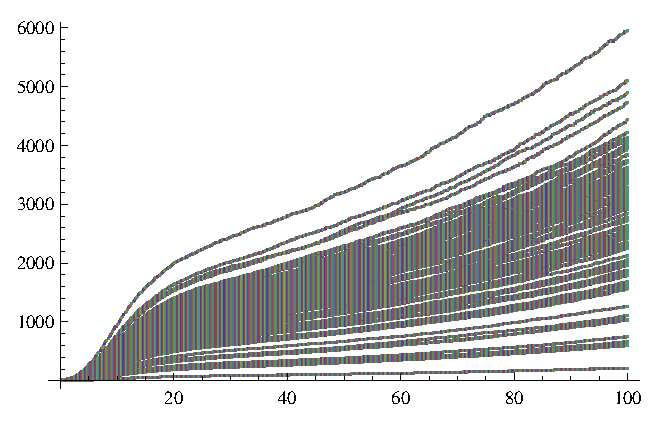
\epsfig{file=graf1prueba.eps,width=.40\textwidth} & 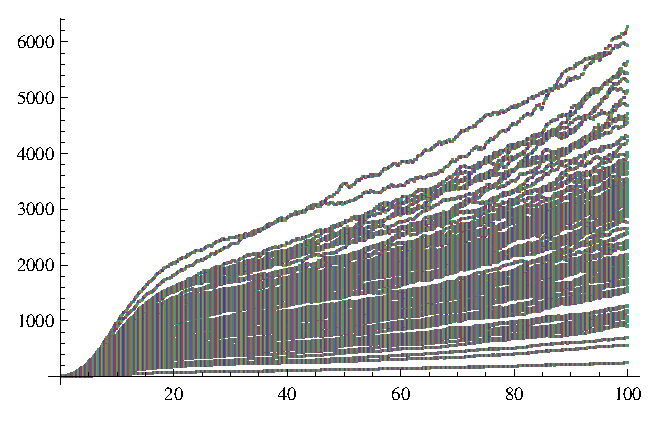
\epsfig{file=graf2prueba.eps,width=.40\textwidth} \\
  $\sigma^2=10^{-5}$ & $\sigma^2=10^{-4}$ \\
  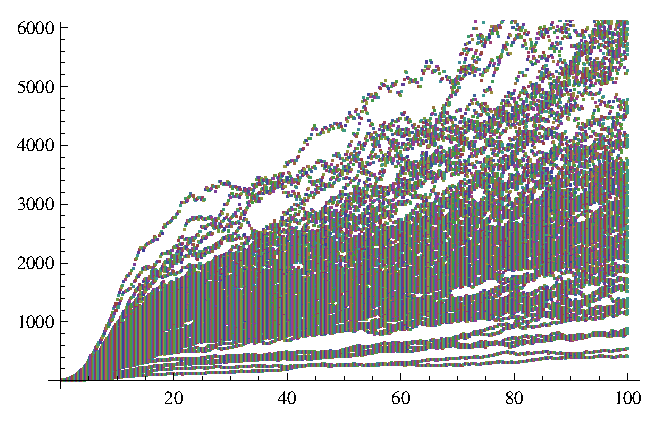
\epsfig{file=graf3prueba.eps,width=.40\textwidth} & 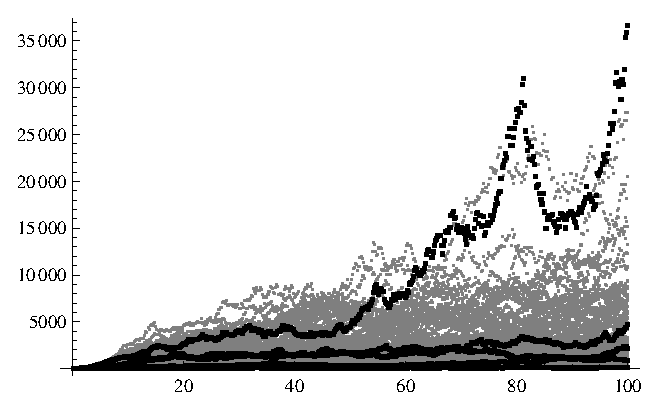
\epsfig{file=graf4prueba.eps,width=.40\textwidth} \\
  $\sigma^2=10^{-3}$ & $\sigma^2=10^{-2}$\\
\end{tabular}
\caption{Simulated paths for Gompertz-lognormal processes from $t_0=1$ to $t_{500}=100$, with values $m=1$, $\beta=0.2$, and $c=0.013$ and different values of noise; $\sigma^2=10^{-5}$, $\sigma^2=10^{-4}$, $\sigma^2=10^{-3}$ and  $\sigma^2=10^{-2}$. Black lines highlight the paths last value $x_{i;500}$ are maximum, minimum and the quartiles of the output range. } \label{1:figura:path}
\end{figure*}

For each set of paths, the five proposed methods are used to estimate the parameters. For each method, we calculate the following error measurements \cite{error}: mean squared error (MSE), mean absolute error (MAE), mean absolute percentage error (MAPE), symmetric mean absolute percentage error (SMAPE) and mean relative absolute error (MRAE). In the case of the MRAE, the error is calculated between the estimated mean function and the path that a simple model gives. In this case a \emph{naive} model is used; the predicted value is equal to the value before it.

We summarize the results in Tables \ref{tabla:parametros}  and \ref{tabla:errores}. All the experiments are repeated 30 times, except IM, which is a deterministic approach. The average of each estimated parameter, using just valid outputs, is calculated later the experimentation process and included in Table \ref{tabla:parametros}.


%maribel quito aqu{\'\i} varias frases para ponerlas m{\'a}s abajo, que creo que tienen m{\'a}s sentido

\begin{table*}
\caption{\footnotesize{Average of the estimates $(\overline{\hat{m}}$, $\overline{\hat{\beta}}$, $\overline{\hat{c}}$, $\overline{\hat{\sigma}^{2}})$; standard deviation of each one ($sd$); average and standard deviation of the value of function (\ref{ecuacion}) ($\overline{\hat{F}},sd$); best found solution (${\hat{F}}_{min}$). Paths simulated with $m=1$, $\beta=0.2$ and $c=0.013$ and $\sigma^2=\{10^{-5},10^{-4},10^{-3},10^{-2}\}$. For each method, the number of the successful solutions (\emph{Succ.}) has been included in the second column.}}
\begin{center}
{\scriptsize
\begin{tabular}{lc|rrrrrrrrrr}
   M & Succ.  & $\overline{\hat{m}}\quad$&$sd\qquad$ &  $\overline{\hat{\beta}}\quad$ &$sd\qquad$ &  $\overline{\hat{c}}\qquad$ &$sd\qquad$ &  $\overline{\hat{\sigma}^{2}}\quad\quad$ &$sd\qquad$& $\overline{\hat{F}}\qquad$  &$sd\qquad$ \\
\hline
\multicolumn{12}{c}{Noise Level $\sigma^2=10^{-5}$} \\

\hline
IM 		& $1$ 	&$1,0076$&$-\qquad$      	    & $0,20034$&$-\qquad$      	&$0,01299$&$-\qquad$    	    &$10*10^{-6}$&$-\qquad$	&$-205013,0$	&$-\qquad$\\
NR		& $12$	&$1,0129$ & $7*10^{-10}$	& $0,20273$&$2*10^{-8}$	&$0,01319$ &$3*10^{-8}$	&$12*10^{-6}$&$7*10^{-11}$	&$-256494,2$	&$2*10^{-6}$	 \\
VNS  	& $30$  &$0,9972$&$1*10^{-2}$    & $0,20398$&$3*10^{-3}$  	&$0,01363$&$8*10^{-4}$  	&$14*10^{-6}$&$5*10^{-6}$	&$-254626,4$	&$2298,7$	 \\
SA 		& $30$  &$1,0129$&$3*10^{-5}$ 	& $0,20273$&$9*10^{-6}$  	&$0,01319$&$3*10^{-7}$ 	&$12*10^{-6}$&$4*10^{-8}$	&$-256494,0$	&$1*10^{-1}$	 \\
EA 		& $30$  &$1,0129$&$2*10^{-4}$		& $0,20273$&$4*10^{-6}$  	&$0,01319$&$1*10^{-6}$ 	&$12*10^{-6}$&$4*10^{-9}$	&$-256494,2$	&$1*10^{-2}$\\
\hline
\multicolumn{12}{c}{Noise Level $\sigma^2=10^{-4}$} \\
\hline
IM 		&$1$	&$1,0144$&$-\qquad$           & $0,19846$&$-\qquad$         &$0,01338$&$-\qquad$      &$10*10^{-5}$&$-\qquad$	& $-194477,8$&$-\qquad$			 \\
NR 	&$21$	&$1,0395$&$3*10^{-8}$     &  $0,20815$&$3*10^{-7}$  &$0,01354$&$4*10^{-7}$  &$12*10^{-5}$&$9*10^{-10}$	& $-199315,7$&$2*10^{-5}$\\
VNS		&$30$	&$0,9970$&$1*10^{-2}$     & $0,20854$&$3*10^{-3}$   &$0,01374$&$1*10^{-3}$  &$12*10^{-5}$&$7*10^{-6}$	& $-199170,7$&$216,6$\\
SA 		&$30$	&$1,0394$&$1*10^{-7}$     & $0,20815$&$1*10^{-5}$   &$0,01354$&$1*10^{-5}$	&$12*10^{-4}$&$7*10^{-8}$	& $-199315,7$&$1*10^{-3}$\\
EA 		&$30$	&$1,0395$&$1*10^{-7}$     & $0,20815$&$1*10^{-5}$   &$0,01354 $&$1*10^{-5}$ &$12*10^{-5}$&$7*10^{-8}$	& $-199315,7$&$8*10^{-4}$\\
\hline
\multicolumn{12}{c}{Noise Level $\sigma^2=10^{-3}$} \\
\hline
IM 		&$1$ 	&$1,1366$	&$-\qquad$    	&$0,22761$	&$-\qquad$    	&$0,01478$	&$-\qquad$    	&$10*10^{-4}$&$-\qquad$	& $-88350,2$	&$-\qquad$\\
NR 	&$14$	&$1,1366$	&$2*10^{-8}$	&$0,22761$	&$9*10^{-8}$	&$0,01478$	&$9*10^{-8}$ 	&$12*10^{-4}$&$2*10^{-12}$	& $-141799,8 $	&$7*10^{-8}$\\
VNS 	&$30$	&$0,9989$	&$1*10^{-2}$	&$0,22737$	&$3*10^{-3}$	&$0,01459$	&$8*10^{-4}$	&$13*10^{-4}$&$1*10^{-5}$	& $-141790,6$	&$10,0$\\
SA 		&$30$	&$1,1366$	&$2*10^{-4}$	&$0,22759$	&$6*10^{-5}$	&$0,01476$	&$2*10^{-5}$ 	&$12*10^{-4}$&$6*10^{-7}$	& $-141799,8 $&$8*10^{-3}$\\
EA 		&$30$	&$1,1366$	&$3*10^{-6}$	&$0,22761$	&$8*10^{-7}$	&$0,01478$	&$1*10^{-7}$ 	&$12*10^{-4}$&$5*10^{-9}$	& $-141799,8$&$4*10^{-6}$\\
\hline
\multicolumn{12}{c}{Noise Level $\sigma^2=10^{-2}$} \\
\hline
IM 		&$0$ 	&$-\quad$&$ -\qquad$    		&$-\quad$&$-\qquad$    			&$-\quad$&$ -\qquad$    			&$-\qquad$&$-\qquad$				 &$-\qquad$			&$-\qquad$		\\
NR 	&$16$	&$1,5472$&$2*10^{-7}$	&$0,32957$&$2*10^{-7}$	&$0,02079$&$2*10^{-6}$ 	&$12*10^{-3}$&$4*10^{-10}$	&$-84972,8$		&$2*10^{-8}$\\
VNS 	&$30$	&$0,9371$&$5*10^{-3}$	&$0,33014$&$2*10^{-3}$	&$0,02081$&$5*10^{-4}$   &$12*10^{-3}$&$4*10^{-5}$ 	&$-84972,3$		&$0.75$		\\
SA 		&$30$	&$1,1366$&$2*10^{-4}$	&$0,22759$&$6*10^{-5}$	&$0,01476$&$2*10^{-5}$ 	&$12*10^{-3}$&$4*10^{-5}$	&$-84965,0$		&$1*10^{-3}$ \\
EA 		&$30$	&$1,5391$&$2*10^{-3}$	&$0,32210$&$6*10^{-4}$	&$0,01560$&$3*10^{-6}$ 	&$12*10^{-3}$&$7*10^{-6}$	&$-84965,1$		&$1*10^{-3}$ \\
\hline
\end{tabular}}
\label{tabla:parametros}
\end{center}
\end{table*}


Table \ref{tabla:parametros} includes the average of the parameters estimations when the noise on the simulation is $10^{-5}$, $10^{-4}$, $10^{-3}$ and $10^{-2}$. We also include the standard deviation because  small changes in the value of the parameters could involve big alterations in objective function results.

%%Desiree
The number of valid outputs is included in the second column of the Table \ref{tabla:parametros}, labelled \emph{Succ.}. Note that NR has been launched $30$ runs, however only some of their outputs, $12$, $21$, $14$ and $16$ times respectively, provides a successful solution.

As can be seen, all the methods provide a solution close to those used in the simulation for each parameter, and the closest is the obtained with the IM for every value of $\sigma^2$ but $\sigma^2 =10^{-2}$, because there is no solution this time using IM. According to this table, all considered methods found good results for the estimations of the parameters in comparison to the values used for the simulation. This table also shows the values with these estimations for the function (\ref{ecuacion}).

Usually, researchers  in bio-inspired algorithms present tables with the means of their algorithm scores. However, in this case, the averaged values in Table \ref{tabla:parametros} are not useful for evaluating function (\ref{ecuacion}) because the means of the scores are not really outputs of the methods. Due to the values of each parameter strongly influence the function value, we decide to select one of the estimated set of parameters, which is included in the left part of Table \ref{tabla:errores}. We select the set of values $\{\hat{m}$; $\hat{\beta}$; $\hat{c}$; $\hat{\sigma}^2 \}$ which minimise the function (\ref{ecuacion}), labelled as $\{\hat{m}_{F_{min}}$; $\hat{\beta}_{F_{min}}$; $\hat{c}_{F_{min}}$; $\hat{\sigma}^2_{F_{min}}\}$, because the goal of this experimentation process is to minimise it.


Table \ref{tabla:errores} includes firstly the selected sets of estimations $\{\hat{m}_{F_{min}}$; $\hat{\beta}_{F_{min}}$; $\hat{c}_{F_{min}}$ ; $\hat{\sigma}^2_{F_{min}}\}$. Secondly, it shows $\hat{F}_{min}$, that is, the values of the function (\ref{ecuacion}) that the selected sets of estimates provide. Finally, it presents the means of the error measurements MSE, MAE, MAPE, SMAPE and MRAE given by each method and the four sets of paths.



\begin{table*}
\caption{\footnotesize{Estimated set of parameters, function (\ref{ecuacion}) it provides and error measurements.}}
\begin{center}
{\scriptsize
\begin{tabular}{c|rrrrr|rrrrr}
\hline
   M & $\hat{F}_{min}\ $ &  $\hat{m}_{F_{min}}$ &  $\hat{\beta}_{F_{min}}$ &  $\hat{c}_{F_{min}}$ & $\hat{\sigma}^{2}_{F_{min}}\ $&  MSE\hspace{0.2cm} &  MAE &  MAPE &  SMAPE & MRAE  \\

\hline
\hline
&\multicolumn{10}{c}{ Noise Level $ \sigma^2= 10^{-5}$} \\
\hline

	 		IM & $-205013$		&$1,008$	&$0,200$	&$0,013$	&$26*10^{-5}$	& $2858$	&$30,52$ 	&$2,10$	&$0,02$	&$39,85$	\\
	 		NR & $-256494$		&$1,013$	&$0,203$	&$0,013$ 	&$13*10^{-6}$ & $2785$	&$28,48$	&$1,87$	&$0,02$	&$32,17$	\\
            VNS & $-256476$		&$0,999$	&$0,203$	&$0,013$    &$13*10^{-6}$	& $14052$	&$94,33$ 	&$5,74$	&$0,06$	&$71,20$	\\
 			SA & $-256494$    	&$1,013$	&$0,203$	&$0,013$   	&$12*10^{-6}$	&$2791$		&$28,51$  &$1,87$	&$0,02$ &$32,18$	\\
 			EA& $-256494$   	&$1,013$	&$0,203$	&$0,013$	&$13*10^{-6}$ 	&$2785$		&$	28,48$	&$1,87$	&$0,02$	&$32,17$ 	\\
 \hline
\hline
&\multicolumn{10}{c}{Noise Level $ \sigma^2= 10^{-4}$} \\
%&\multicolumn{5}{|c||}{Non-trimmed}&\multicolumn{5}{c|}{Trimmed} \\
\hline
	 	    IM & $-148757$		&$1,017$	&$0,198$	&$0,013$	&$244*10^{-5}$	&$51123$ 	&$146,42$ 	&$10,70$ 	&$0,10$	&$129,92$	\\
	 	    NR& $-199316$		&$1,039$	&$0,208$	&$0,014$	&$12*10^{-5}$ &$25027$	&$87,14$	&$5,43$		&$0,05$	&$73,73$ 	\\
            VNS& $-199315$		&$0,999$	&$0,208$	&$0,014$	&$13*10^{-5}$	&$154407$ 	&$300,77$ 	&$17,88$ 	&$0,20$	&$232,38$	\\
 			SA& $-199316$		&$1,039$	&$0,208$	&$0,014$	&$12*10^{-5}$ 	&$25025	$	&$87,13	$	&$5,43$		&$0,05$	&$73,73$	\\
 			EA & $-199316$		&$1,039$	&$0,208$	&$0,014$	&$12*10^{-5}$	&$25027$	&$87,14$	&$5,43$		&$0,05$	&$73,73$	\\
\hline
\hline
&\multicolumn{10}{c}{Noise Level $ \sigma^2= 10^{-3}$} \\
%&\multicolumn{5}{|c||}{Non-trimmed}&\multicolumn{5}{c|}{Trimmed} \\
\hline
 			IM&$-88517$	&$1,035$	&$0,186$	&$0,022$	&$275*10^{-4}$ 	&$16443800$	&$2262,92$ 	&$146,54$	&$0,75$		&$725,20$	\\
 			NR&$-141800$	&$1,137$	&$0,228$	&$0,015$	&$13*10^{-4}$ &$341403$		&$267,03$	&$15,88$	&$0,16$		&$71,62$	\\
           VNS &$-141800$	&$0,999$	&$0,228$	&$0,015$	&$13*10^{-4}$	&$1461321$	&$867,30$ 	&$44,93$	&$0,60$		&$208,52$	\\
 			SA &$-141800$	&$1,136$	&$0,228$	&$0,015$	&$13*10^{-4}$	&$340903$		&$266,83$	&$15,88$	&$0,16$		&$71,60$	\\
 			EA &$-141800$	&$1,137$	&$0,228$	&$0,015$	&$13*10^{-4}$	&$341403$		&$267,03$	&$15,88$	&$0,16$		&$71,62$	\\
\hline
\hline
&\multicolumn{10}{c}{Noise Level $\sigma^2=  10^{-2}$} \\
%&\multicolumn{5}{|c||}{Non-trimmed}&\multicolumn{5}{c|}{Trimmed} \\
\hline
 			IM 	&$-\ \ \ $				& $-\ \ $ 		&$-\ \ $		&$-\ \ $		& $-\ \ \ \ \ $		& $-\ \ \ \ $		&$-\ \ \ $		&$-\ \ $		 &$-\ \,$		&$-\ \ \,$\\
 			NR&$-84973$	&$1,547$	&$0,330$	&$0,021$	&$12*10^{-3}$ &$5120383$			&$955,6$	&$79,18$	&$0,54$		& $139,8$	\\
            VNS&$-84973$	&$0,939$	&$0,330$	&$0,021$	&$12*10^{-3}$	&$9921164$	& $1785,9$ 	&$78,32$	&$1,34$		& $136,7$	\\
 			SA &$-84965$	&$1,540$	&$0,322$	&$0,016$	&$12*10^{-3}$	&$5642929$			&$1010,4$	&$62,19$	&$0,54$	&$108,9$	\\
 			EA &$-84965$	&$1,539$	&$0,322$	&$0,016$	&$12*10^{-3}$	&$5634217$		&$1009,3$	&$62,29$	&$0,53$	&$109,1$	\\
\hline
\end{tabular}
}
\label{tabla:errores}\end{center}
\end{table*}

\section{Conclusions}
\label{sec:Conclusion}

Table \ref{tabla:parametros} shows that the IM provides an estimated set of parameters which is the closets to the used in simulation, excepting for $\sigma^2=10^{-2}$, where the method is not able to provide a solution. In spite of that, the values of function (\ref{ecuacion}) to minimise, with those estimations, are the highest in all cases. Moreover, error measurements, shown in Table \ref{tabla:errores}, for IM are not the lowest in any case. The main advantage of IM is it spends less time than the rest of the methods and it always gives the same solution.

Newton-Raphson method provides or not a solution depending on the starting point. When it is not good enough the method diverges, but when the initial value is close to the real one, the method provides a precise solution. In Table \ref{tabla:parametros} appears data about the number of successfully runs (\emph{Succ.}) for each noise level; 12, 21, 14 and 16 respectively in the simulation study. For the success cases, the means of the estimations obtained for the parameters are close to the values used in simulation, as well as results given by SA and EA methods. The function (\ref{ecuacion}) evaluated with the estimations has, in mean, the lowest value, and the reached minimum is the lowest too, together with SA and EA methods. Despite the means and the minimum in these tree methods are close each other, NR is the one that presents lower standard deviation, thus the results are closer using NR than using SA or EA.

Table \ref{tabla:errores} shows that the better found solution (which minimise the function (\ref{ecuacion})) for NR is similar to the provided by EA and SA. The estimated set of parameters, value of function (\ref{ecuacion}) reached and error measurements are very close for low noise and not much far for higher noise. Thus, the error measurements are not better nor worse than the results provided by EA or SA methods. The advantage of NR is that, if you have some knowledge about the expected solution, this method provides an exact solution in a few seconds. The drawback is that the method is not as reliable as the others.

Based on the values in (Table \ref{tabla:parametros}), we note that VNS method gets competitive average values comparing them with the other methods, but the standard deviations obtained for all the estimations are high. It implies that the method varies in the solutions provided much more than the others methods. Hence, in Table \ref{tabla:errores} appears that VNS presents the highest error values almost always. Only for high noise level, IM gives worse results.

As we commented before, generally, SA and EA provide similar results to NR. For low noise cases, we can not appreciate any difference but, when data show high noise SA and EA provide different mean estimations for the parameters from NR and higher value of function (\ref{ecuacion}).
These bio-inspired methods do not need any previous knowledge about the objective function and they supply competitive solutions for all the runs. Nevertheless, SA and EA are slower than the other considered methods, and in Table \ref{tabla:parametros} the main difference we appreciate between EA and SA is that the standard deviation for the $\overline{\hat F}$ is lower for EA. Otherwise, NR and EA obtain the same parameter estimations, which minimise function (\ref{ecuacion}) and are very similar to EA ones. In Table \ref{tabla:errores} we can see similar behaviour. For hight noise level, EA and SA provide different results with respect to NR, and they have less average errors MAPE, SMAPE and MRAE than NR but higher error MSE and MAE.





In short, the IM allows us, when no high noise is present, to estimate the parameters close to the real set, although it does not mean the function estimated looks like the observed path. In terms of errors and likelihood value, the NR method gives as good results as EA and SA, but only EA or SA provides always successful results. For high noise, bio-inspired algorithms give results more reliable than IM, NR or VNS give although they are less exact for high noise levels. VNS is not better than other methods in any case.


As future lines we proposes to apply the reliable methods, EA or SA, to model some processes of disease transmission, as influenza dissemination process.




\section*{Acknowledgements}


Hidden for double-blind review

%The authors would like to thank the FEDER of European Union for financial support via project ``Sistema de Informaci{\'o}n y Predicci{\'o}n de bajo coste y aut{\'o}nomo para conocer el Estado de las Carreteras en tiempo real mediante dispositivos distribuidos" (SIPEsCa) of the ``Programa Operativo FEDER de Andaluc\'{i}a 2007-2013". We also thank all Agency of Public Works of Andalusia Regional Government staff and researchers for their dedication and their professionalism. This work has been supported in part by project ANYSELF (TIN2011-28627-C04-02) and MICINN (Spain) MTM2011-28962.
%\begin{figure}
%\begin{center}
%
\epsfig{file=sipesca_2.eps,width=4cm}
%\end{center}
%\end{figure}
\bibliographystyle{abbrv}
\bibliography{paperGecco}
\end{document}
